\section{Instalar Debian Bookworm}
En esta sección veremos cómo instalar el sistema operativo bookworm a una raspbery pi.

Lo primero que debemos hacer es comprar una \textbf{micro sd} (aprox de 32 GB). Luego, instalar en nuestra computadora el programa \href{https://www.raspberrypi.com/software/}{Raspberry Pi Imager}, el cual se puede instalar desde \href{https://www.raspberrypi.com/software/}{acá}.

Para instalar Raspbery Pi Imager en linux, procederemos a instalar el AppImage. En la página seleccionamos "Download for Linux (x86\_64)".

\begin{figure}[H]
    \centering
    \makebox[\textwidth][c]{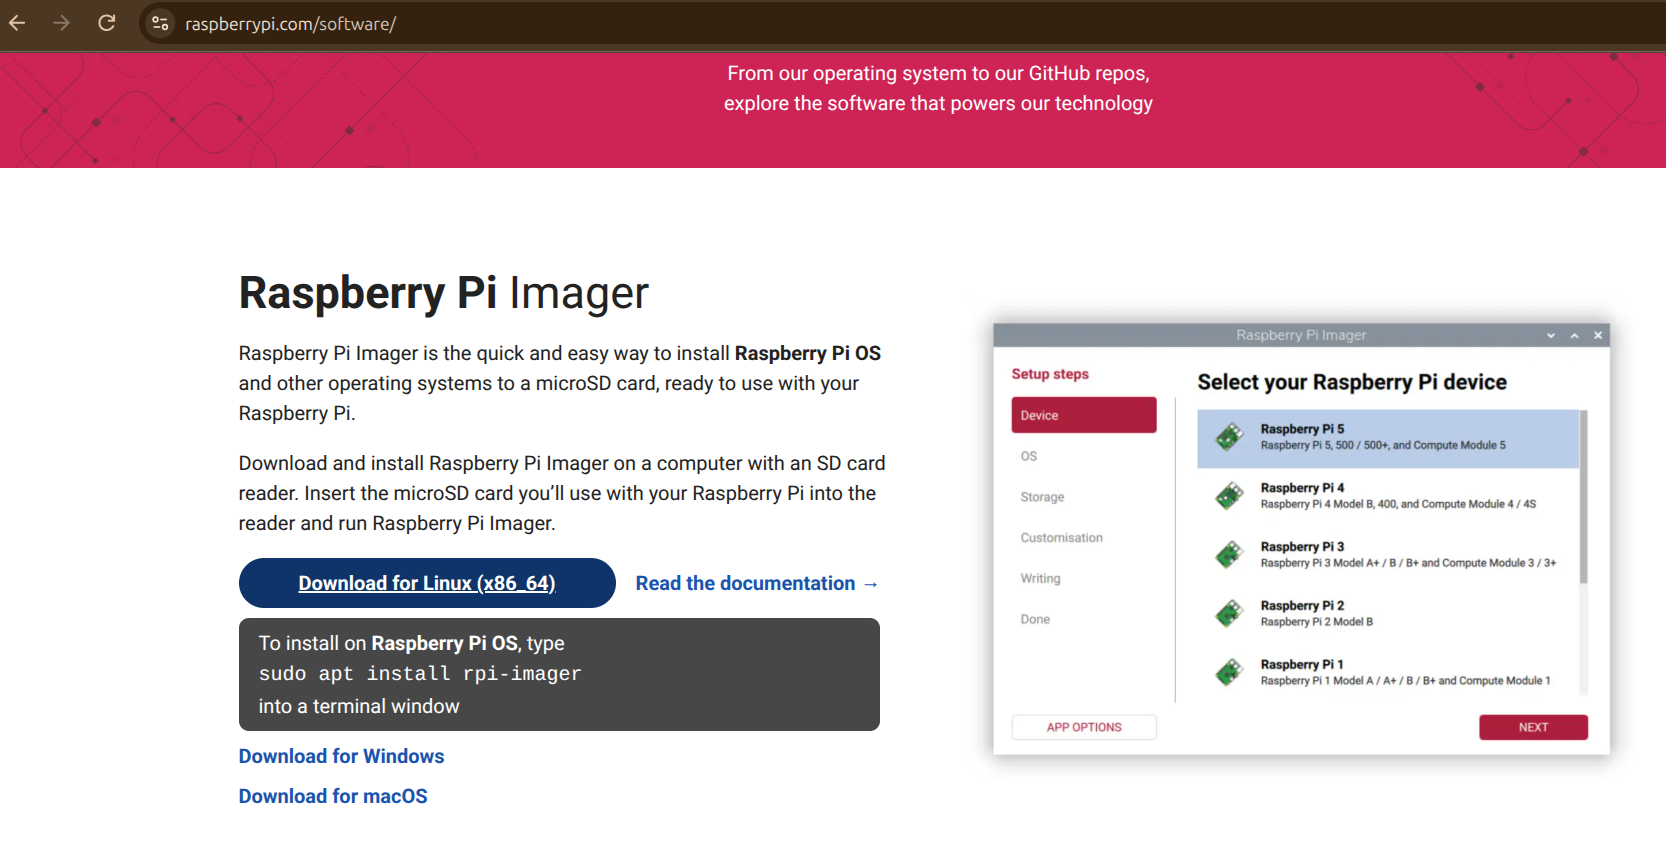
\includegraphics[width=1.2\textwidth]{imagenes/image.png}}
    \caption{Seleccionamos Download for Linux (x86-64)}
    \label{fig:mi_imagen}
\end{figure}

Y así tendremos nuestro AppImage en la carpeta de Descargas (o Downloads):

\begin{figure}[H]
    \centering
    \makebox[\textwidth][c]{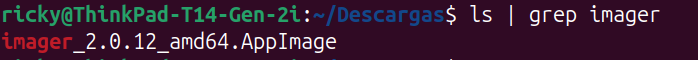
\includegraphics[width=1.2\textwidth]{imagenes/image2.png}}
    \caption{AppImage en Descargas}
    \label{fig:mi_imagen}
\end{figure}

Procedemos a dar permisos de ejecución para todos sobre el AppImage con el comando \texttt{chmod a+x imager\_2.0.12\_amd64.AppImage}.

\begin{figure}[H]
    \centering
    \makebox[\textwidth][c]{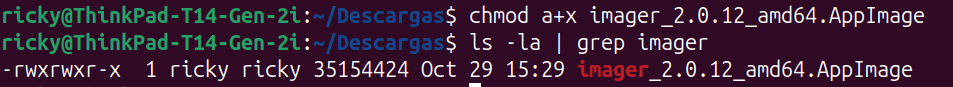
\includegraphics[width=1.2\textwidth]{imagenes/image3.png}}
    \caption{Otorgamos permisos de ejecución.}
    \label{fig:mi_imagen}
\end{figure}

Ahora ejecutamos el archivo con \texttt{./imager\_2.0.12\_amd64.AppImage}.

\begin{figure}[H]
    \centering
    \makebox[\textwidth][c]{
\includegraphics[width=1.2\textwidth]{imagenes/image4.png}}
    \caption{Ejecutamos el AppImage}
    \label{fig:mi_imagen}
\end{figure}

Al abrir, seleccionamos \textbf{INSTALL AUTHORIZATION}.

\begin{figure}[H]
    \centering
    \makebox[\textwidth][c]{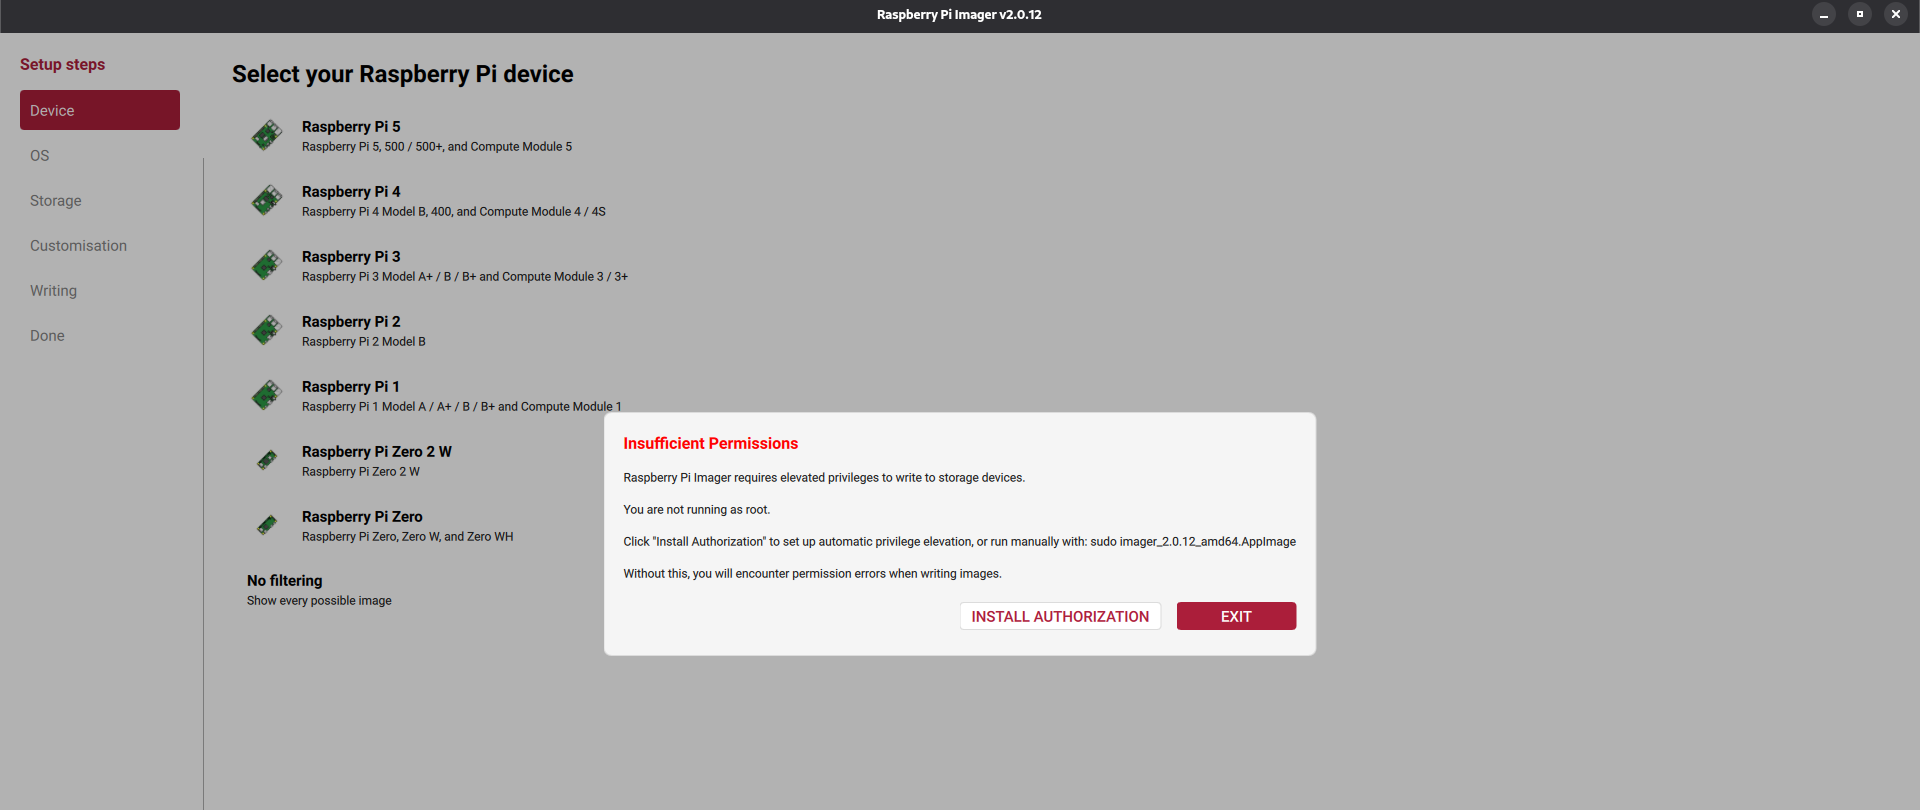
\includegraphics[width=1.2\textwidth]{imagenes/image5.png}}
    \caption{Seleccionamos Install Authorization.}
    \label{fig:mi_imagen}
\end{figure}

Hasta el momento, los paquitos trabajan con la raspbery pi 4, así que seleccionamos \textbf{Raspberry Pi 4} y damos click en next.

\begin{figure}[H]
    \centering
    \makebox[\textwidth][c]{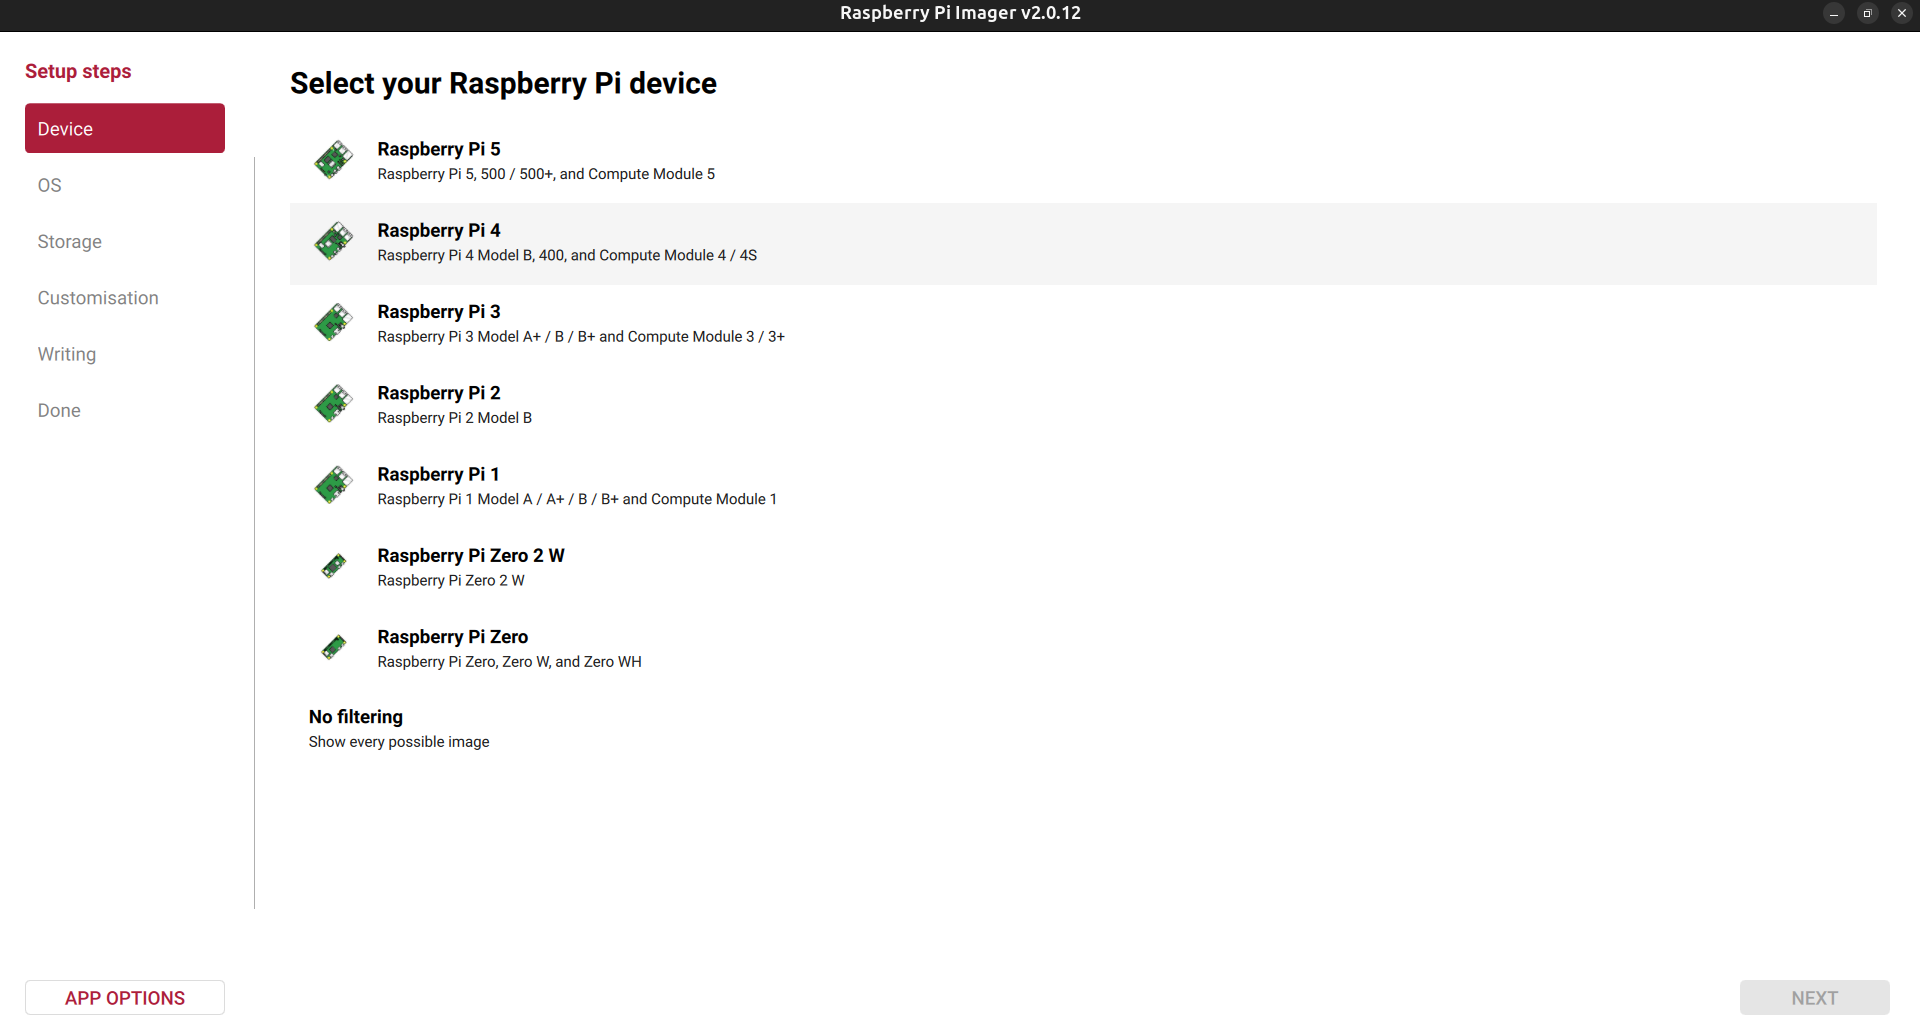
\includegraphics[width=1.2\textwidth]{imagenes/image6.png}}
    \caption{Seleccionamos Raspberry Pi 4, y damos click en next.}
    \label{fig:mi_imagen}
\end{figure}

Al elegir el sistema operativo a instalar en la raspberry, seleccionamos \textbf{Raspberry Pi OS (other)}.

\begin{figure}[H]
    \centering
    \makebox[\textwidth][c]{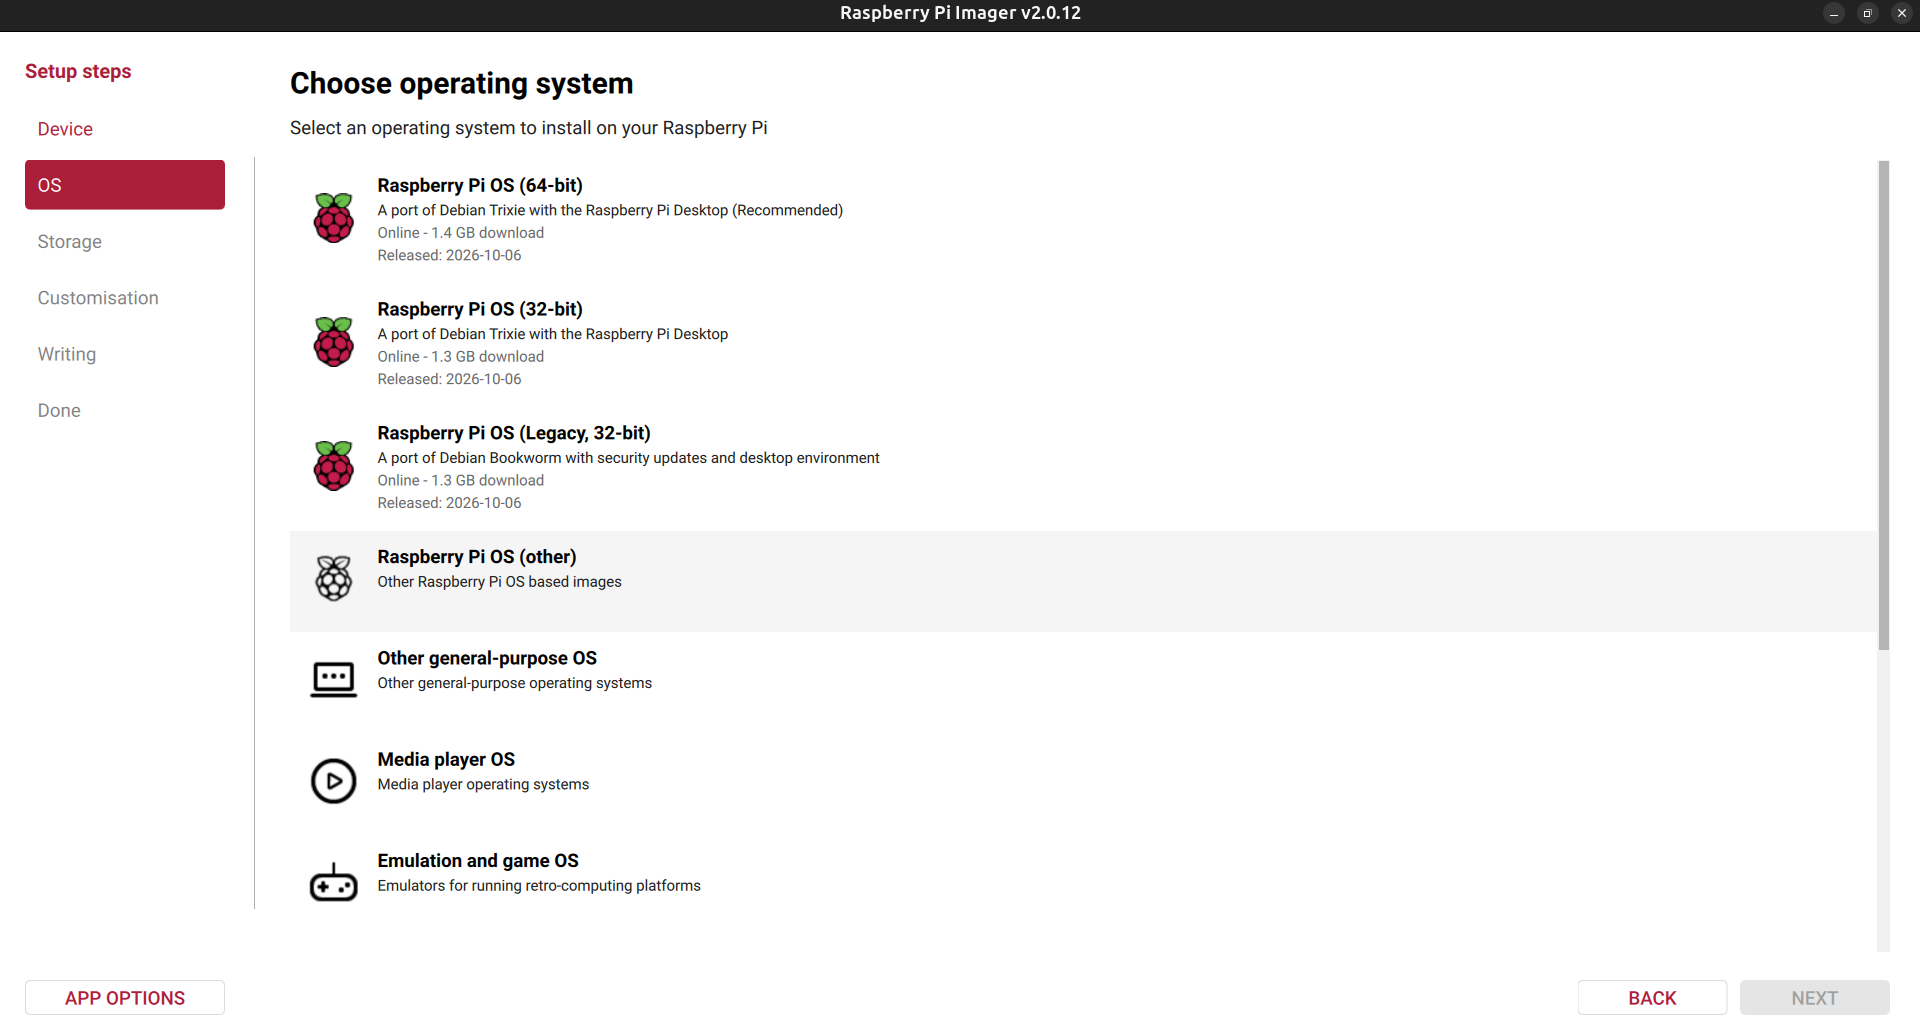
\includegraphics[width=1.2\textwidth]{imagenes/image7.png}}
    \caption{Seleccionamos Raspberry Pi OS (other).}
    \label{fig:mi_imagen}
\end{figure}

Luego, seleccionamos la opción \textbf{Raspberry Pi OS (Legacy, 64-bit)} \textit{A port of Debian Bookworm with security updates and desktop environment}. 

\begin{figure}[H]
    \centering
    \makebox[\textwidth][c]{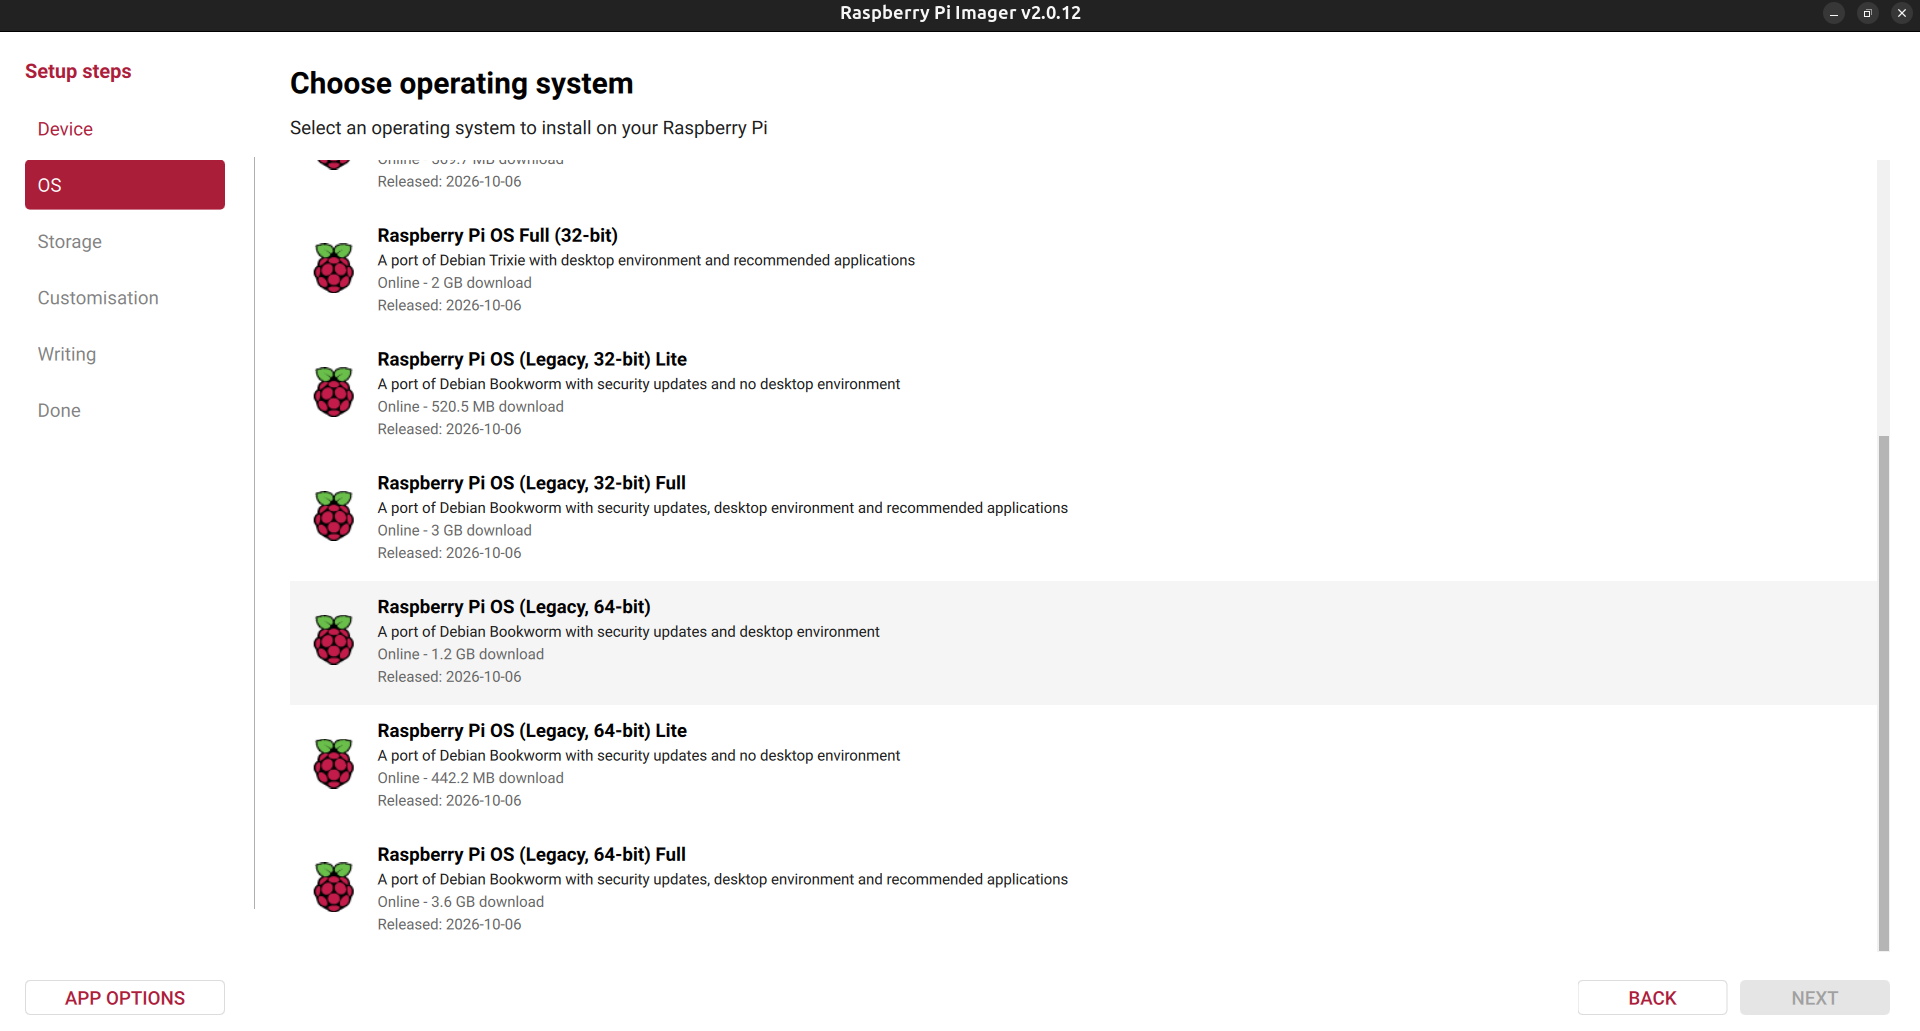
\includegraphics[width=1.2\textwidth]{imagenes/image8.png}}
    \caption{Seleccionamos \textbf{Raspberry Pi OS (Legacy, 64-bit)}.}
    \label{fig:mi_imagen}
\end{figure}
 
Para los paquitos, tenemos la instalación de ROS 2 para Bookworm, esta versión del sistema operativo no es tan pesada y tiene entorno de escritorio. Hemos visto también que con otras versiones no se muestra el escritorio (cuando supuestamente sí debería mostrarlo). 

\begin{figure}[H]
    \centering
    \makebox[\textwidth][c]{
\includegraphics[width=0.5\textwidth]{imagenes/bookworm.png}}
    \caption{Bookworm, Debian 12.}
    \label{fig:mi_imagen}
\end{figure}

Luego, insertamos el micro SD a nuestra computadora (ya sea directamente o con un adaptador a USB), e iniciamos la descarga. 

Una vez que tenemos instalado el sistema operativo \textit{bookworm} en el micro SD, lo insertamos en la raspberry pi en su puerto para micro SD. 

\begin{figure}[H]
    \centering
    \makebox[\textwidth][c]{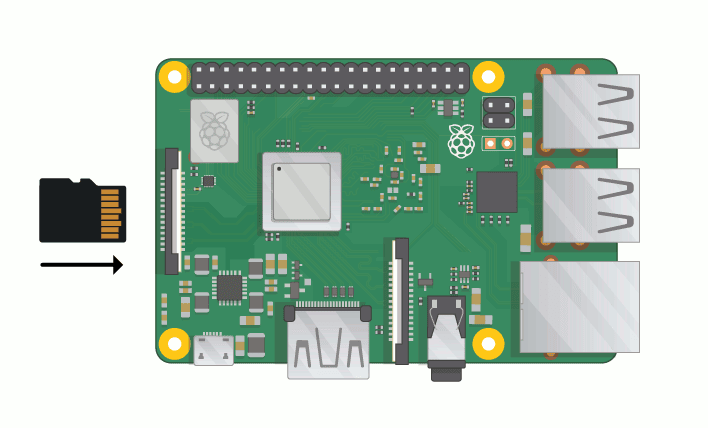
\includegraphics[width=0.9\textwidth]{imagenes/microsd-raspberry.png}}
    \caption{Ubicación y orientación de micro SD en raspberry.}
    \label{fig:mi_imagen}
\end{figure}

